\begin{figure*}[t]
    \centering
    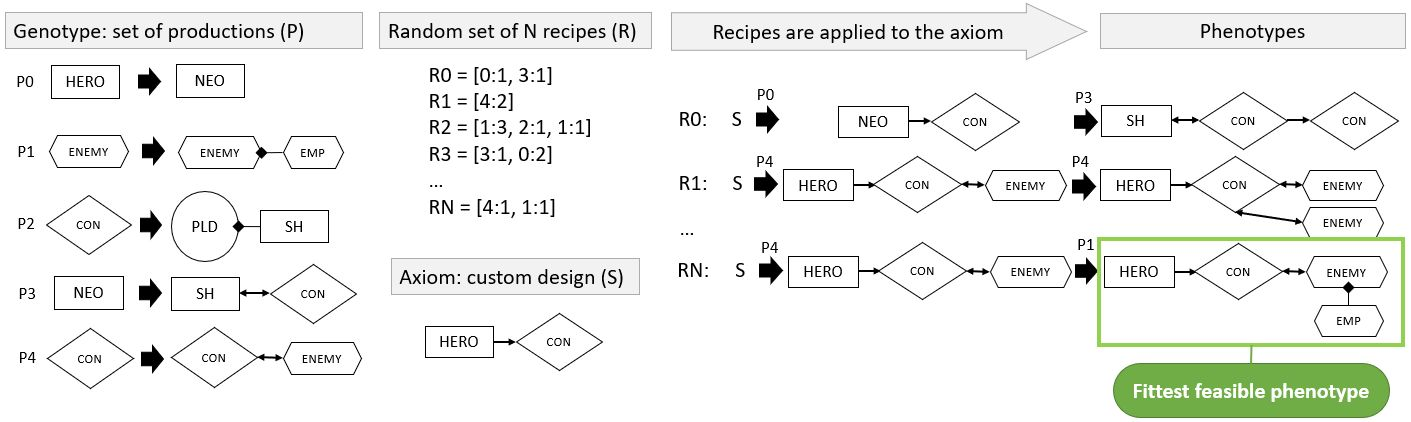
\includegraphics[width=\textwidth]{figures/gen2seq.jpg}
    \caption{sample complete process from an individual's genotype to the phenotype.}
    \label{fig:gen2phen}
\end{figure*}


% Actually, all of this could easily be a new chapter.
\subsection{Evolving Narratives with Graph Grammars} \label{sec:evolvingNarratives}

We use the Constrained MAP-Elites~\cite{p12Khalifa2018}, and adapt it to work with graph grammars, evolve production rules, and adapt the evolution towards a target similar to~\cite{p12Alvarez2020-ICMAPE}. Constrained MAP-Elites adds feasible-infeasible two populations to each cell, effectively evolving sub-populations per cell. An individual's phenotype is a narrative graph, and its encoding genotype is the production rules of a graph grammar. A graph grammar is a context-free grammar whose productions add, remove, and modify nodes and edges of a graph. Our implementation uses the tropes listed in Table \ref{tab:tropes} as nodes, and the three available connection types as edges ($\rightarrow$, $\leftrightarrow$, $\diamondsuit$--). Graph grammars do not apply rules sequentially; instead, every individual does a random sampling of the rules in their genotype to produce \emph{recipes} to generate graphs. \emph{Recipes} describe the rules' order and repetition, and their size is limited by the amount of production rules as minimum and the minimum plus five as maximum. \emph{Recipes} do not have repetitions within them, i.e., if rule 1 is added at step 2, subsequent addition would simply add to the number of times that rule will be applied at step 2. Their size is limited by the number of production rules as minimum and up to five more samples as maximum. Figure~\ref{fig:gen2phen} shows a sample complete process from an individual's genotype (i.e., rules) to the phenotype (i.e., narrative graph).

%The EA manages an infeasible and feasible population within each cell~\cite{p12Kimbrough2008}. 

Individuals move between the feasible and infeasible population depending on the feasibility constraint. NGs are deemed infeasible if the nodes are not fully connected or if there exists a conflict pattern with more than one self-conflict. Infeasible individuals are evaluated based on how close they are to be fully connected and not having any inadequate self-conflict. The fitness function assesses NGs that are deemed feasible based on their coherence (equation~\ref{eq:coherence_fitness}), which we use to assess how correct, coherent, and in general, syntactically correct the narrative graphs are. Coherence aims at maximizing an equally weighted sum between cohesion and consistency. Cohesion refers to the link between elements that hold together to form some group. In our implementation, it focuses on minimizing the number of auxiliary patterns by calculating the proportion of \emph{Nothing} and \emph{Broken Link} among all patterns in NG. A consistent NG should be regular and free of contradictions. Thus, we calculate \emph{consistency} (eq.~\ref{eq:consistency_fitness}) as the collective quality of micro-patterns since they are the building blocks, and conflicts' goodness based on the number of fake conflicts. Thus, we aim at maximizing the quality of micro-patterns and minimizing contradictions created by meso-patterns.

%In effect, with consistency, we aim to maximize the quality of micro-patterns and minimize contradictions created by meso-patterns . %It is important, as well, to highlight that these and subsequent metrics are heuristics developed to evaluate the graphs, but they do not stand in or replace human judgement. 

%These and subsequent metrics are not evaluated with humans; thus, they do not stand in or replace human judgement, and they are just heuristics . 


\begin{equation}
\label{eq:consistency_fitness}
f_{consistency} = \frac{\sum_{i=0}^{len(ng_{micro})} i_{qual}}{len(ng_{micropat})} -  \\ 
\frac{len(ng_{fakeConfP})}{len(ng_{confP})} 
\end{equation}

\begin{equation}
\label{eq:coherence_fitness}
f_{coherence} = f_{consistency} + (1.0 - f_{cohesion})
\end{equation}

Furthermore, MAP-Elites uses behavioral dimensions in a grid shape to retain and foster diversity throughout generations. We use the following two dimensions to evaluate the diversity: 

\textbf{Step.} Step (eq.~\ref{eq:StepDim}) calculates the Levenshtein distance~\cite{p12Levenshtein96-editDistance} between two narrative graphs, taking into consideration the number and type of nodes and connections. Step is normalized using step threshold $\theta = 11$ determined through a process of experimentation, which does not consider steps farther than $\theta$, avoiding the generation of too dissimilar graphs.

\begin{equation}
\label{eq:StepDim}
D_{step} =  \min (lev_{EG,RG} (|EG|, |RG|), \theta)
\end{equation}

\textbf{Interestingness (int).} We aim at measuring the semantic quality of a narrative graph. A narrative graph can be syntactically correct and coherent yet lack a good semantic quality and do not evoke interest for designers or players. Therefore, we leverage \textbf{plot point}, \textbf{plot twist}, and \textbf{active plot device} patterns to measure the \emph{interestingness} of the NGs. The nature of \emph{interestingness} creates pressure on the fitness function since the incidence of the three meso-patterns could (if overused) ``degenerate'' the narrative; thus, decreasing its coherence. $D_{int}$ is calculated as the weighted sum ($w_{0}=0.4, w_{1}=0.2, w_{2}=0.4$) of the normalized cumulative quality of \textbf{APDs}, \textbf{PPs}, and \textbf{PTs} within an NG (eq.~\ref{eq:interesting_fitness}).

\begin{equation}
\label{eq:interesting_fitness}
D_{int} = w_{0} \times \frac{APD_{q}}{\#APD} + w_{1} \times \frac{\#PP_{q}}{\#PP} +  w_{2} \times \frac{PT_{q}}{\#PT}
\end{equation}

%These metrics are not evaluated with humans; thus, they do not stand in or replace human judgement. 


%which we have to set the system 

%In future work, we aim at validating them with human designers

%, and they just serve as proxies. They arWe aim at validating them in future work and combine 

%the quality is an estimated heuristic based on their functionality and relation to other similar patterns. We agree with the description done by R1, but these qualities are relative to the edited graph. We envision these as parameterized qualities, as one of our goals with the system is to create a mixed-initiative system where qualities will be adapted to what the designer creates.

%during
%system development we need to be able to tune the graph outputs without humans in the loop, so we are using X/Y/Z arbitrary metrics that we've found to work and which we plan to validate against human
%judgements later

\subsubsection{Experiments}

% \begin{table}[t]
% \label{tab:algorithm_info}
% \caption{Table captions should be placed above the
% tables.}\label{tab1}
% % \renewcommand{\arraystretch}{1.2}
% \setlength{\tabcolsep}{4pt}
% \resizebox{\textwidth}{!}{%
% \begin{tabular}{|l|l|l|l|l|}
% \hline
% Target Graph & Coverage (\%) & Avg. Fitness & QD-Score & Interestingness\\
% \hline
% Zelda: OoT (fig.\ref{fig:teaserfig}.a)          & 20.9$\pm$0.02 & 0.65$\pm$0.00 & 131.96$\pm$5.86 & 0.39$\pm$0.02\\
% Zelda: LttP (fig.\ref{fig:teaserfig}.b)         & 21.1$\pm$0.00 & 0.70$\pm$0.00 & 170.22$\pm$10.65 & 0.38$\pm$0.01 \\
% Super Mario Bros (fig.\ref{fig:teaserfig}.c)    & 21.1$\pm$0.01 & 0.69$\pm$0.00 & 137.82$\pm$36.04 & 0.36$\pm$0.02\\
% \hline
% \end{tabular}
% }%
% \end{table}

% Please add the following required packages to your document preamble:
% \usepackage{graphicx}

% \caption{Comparative results between target graphs (RG - fig~\ref{fig:teaserfig}, top row) and generated elites (fig~\ref{fig:teaserfig}, bottom row) using MAP-Elites}

% Please add the following required packages to your document preamble:
% \usepackage{graphicx}
\begin{table}[t]
\caption{Comparative results between root graphs and generated elites (shown in fig. \ref{fig:teaserfig})}
\resizebox{\columnwidth}{!}{%
\begin{tabular}{|l|c|c|c|c|}
\hline
Graph                        & \multicolumn{1}{l|}{Cohesion} & \multicolumn{1}{l|}{Consistency} & \multicolumn{1}{l|}{Coherence (fitness)} & \multicolumn{1}{l|}{Interestingness} \\ \hline
RG (fig \ref{fig:teaserfig}.a1)    & 1.0                           & 0.66                             & 0.825                                     & 0.61                                 \\
Elite (fig \ref{fig:teaserfig}.a2) & 1.0                           & 0.76                             & 0.875                                     & 0.73                                 \\ \hline
RG (fig \ref{fig:teaserfig}.b1)    & 1.0                           & 0.75                             & 0.87                                     & 0.38                                 \\
Elite (fig \ref{fig:teaserfig}.b2) & 1.0                           & 0.91                             & 0.95                                    & 0.55                                 \\ \hline
RG (fig \ref{fig:teaserfig}.c1)    & 1.0                           & 0.77                             & 0.88                                     & 0.4                                  \\
Elite (fig \ref{fig:teaserfig}.c2) & 1.0                           & 0.85                             & 0.92                                     & 0.52                                 \\ \hline
\end{tabular}
}
\label{tab:best-generated}
\end{table}



We conducted a series of experiments to evaluate and analyze how the system could evolve NGs into quality-diverse and valid narrative structures. We evolved the three manually constructed narrative graphs shown in figure~\ref{fig:teaserfig}, top row. They were used as root graphs and axioms in the EA, and we used \textit{interestingness} and \textit{step} as behavioral dimensions. We did $5$ MAP-Elites runs per narrative graph, ran each for $500$ generations, and set the initial population to $1000$ randomly created individuals. The initial population is generated by randomly creating between two and five production rules. Each feasible and infeasible population per cell has $25$ individuals. Each individual is limited to test $10$ recipes regardless of the chromosome size. Offspring were produced either by selecting either the left-side or right-side of a random production rule and exchanging them or with a $50$\% mutation chance. If an offspring was generated by mutation, there was a $10$\% chance to add or remove a production rule and a $90$\% to modify in various ways existing production rules.

%We calculated the \textit{coverage}: how much of the constrained search space is explored (i.e., constrained by the behavioral dimensions); the avg. fitness and the avg. interestingness of the population. All runs, regardless of the Root Graph, performed similarly with an avg. of 21\% coverage, 0.68 avg. fitness, and 0.38 avg. interestingness. These results exemplify both the hard task of generating narrative graphs and exploring the possibility space, and the seemingly competing qualities of coherence (i.e., fitness) and interestingness. 

We calculated the \textit{coverage}: how much of the constrained search space is explored (i.e., constrained by the behavioral dimensions); the avg. fitness and the avg. interestingness. All experiments had little variation regarding these metrics, and got in avg. 23.5\% coverage (24.9\%, 21.4\%, and 24.2\%, respectively), 0.79 fitness (0.76, 0.8, 0.8, respectively), and 0.37 interestingness (0.39, 0.37, 0.36, respectively). These results exemplify both the hard task of generating narrative graphs and exploring the possibility space, and the seemingly competing qualities of coherence (i.e., fitness) and interestingness. 

%The experiments got in avg. 23.5\% coverage, 0.79 fitness, and 0.37 interestingness. There was little variation in 

%All runs, regardless of the Root Graph, performed similarly with an avg. of 21\% coverage, 0.68 avg. fitness, and 0.38 avg. interestingness. These results exemplify both the hard task of generating narrative graphs and exploring the possibility space, and the seemingly competing qualities of coherence (i.e., fitness) and interestingness. 

Furthermore, in figure~\ref{fig:teaserfig}, bottom row, it is shown three different example elite narrative graphs, generated from their respective root graphs on the top row and with each individual evaluation shown in table~\ref{tab:best-generated}. The root graphs have a cohesion of 1.0 since none of them have unused nodes or connections and have similar mid-high consistency values because of using generic nodes (e.g., HERO or ENEMY), repeating them, and low involvement in structures by characters. In the case of fig \ref{fig:teaserfig}.a1, the \textbf{RevP} from HERO to SH creates some fake conflicts, which affect the consistency but also boost the interestingness value of the narrative graph. Both fig \ref{fig:teaserfig}.b1 and \ref{fig:teaserfig}.c1, are evaluated similarly with low interestingness; c1 involves a simplistic and linear structure, and b1, while in principle more complex, is also a relatively linear structure with no \textbf{PTs}.

%We calculated the \textit{coverage}: how much of the constrained search space is explored (i.e., constrained by the behavioral dimensions); the avg. fitness and the avg. interestingness of the population. All runs, regardless of the Root Graph, performed similarly with an avg. of 21\% coverage, 0.68 avg. fitness, and 0.38 avg. interestingness. These results exemplify both the hard task of generating narrative graphs and exploring the possibility space, and the seemingly competing qualities of coherence (i.e., fitness) and interestingness. 

%Furthermore, in figure~\ref{fig:teaserfig}, bottom row, it is shown three different example elite narrative graphs, generated from their respective root graphs on the top row and with each individual evaluation shown in table~\ref{tab:best-generated}. The root graphs have a cohesion of 1.0 since none of them have unused nodes or connections and have similar mid-high consistency values because of using generic nodes (e.g., HERO or ENEMY), repeating them, and low involvement in structures by characters. In the case of fig \ref{fig:teaserfig}.a1, the \textbf{RevP} from HERO to SH creates some fake conflicts, which affect the consistency but also boost the interestingness value of the narrative graph. Both fig \ref{fig:teaserfig}.b1 and \ref{fig:teaserfig}.c1, are evaluated similarly with low interestingness; c1 involves a simplistic and linear structure, and b1, while in principle more complex, is also a relatively linear structure with no \textbf{PTs}.

Furthermore, all the exemplar elites have better \textit{consistency}, \textit{coherence}, and \textit{interestingness} than the respective root graph. In figure~\ref{fig:teaserfig}.a2, the graph has been reduced towards a bottleneck, \textbf{RevP} (HERO $\rightarrow$ SH) is removed, and MCG is added as the objective for SH, which could point towards competition or cooperation to enable NEO. Such a change gives more \textit{consistency} to the graph while seemingly reducing its \textit{interestingness}, but this relation and the $\diamondsuit$-- connection between MCG and NEO increase its \textit{interestingness}. In figure~\ref{fig:teaserfig}.b2, the narrative has more interaction between \textbf{Plot Devices}, and the BAD has a more active role. Particularly, the fact that now HERO $\rightarrow$ MCG $\diamondsuit$-- BAD and MHQ $\diamondsuit$-- CHK $\diamondsuit$-- BAD could enable and force the HERO towards two main objectives before overcoming the boss, which is reflected in the higher \textit{Interestingness}. Finally, in figure~\ref{fig:teaserfig}.c2, the narrative did not change much (only four steps away), yet the graph is seemingly better, and the narrative could be very different. The graph has broken the loop which connected DRAKE $\diamondsuit$-- BAD, and could could point towards a side objective. Further, the connection between BAD and MCG has been reversed; thus, the HERO does not need to face the BAD to get the MCG, rather reaching the MCG will have as a consequence the emergence of the BAD. Finally, BAD is no longer connected to EMP and DRAKE; thus, BAD could be its own enemy faction, in this case, complexifying the narrative and creating more challenge.